Mauris pharetra et ultrices neque ornare aenean. Nascetur ridiculus mus mauris vitae ultricies. Placerat orci nulla pellentesque dignissim enim sit amet. Quis risus sed vulputate odio ut. Semper feugiat nibh sed pulvinar proin gravida hendrerit lectus. Nec feugiat nisl pretium fusce id velit ut tortor. Non quam lacus suspendisse faucibus interdum posuere lorem. Lorem sed risus ultricies tristique nulla. Non sodales neque sodales ut etiam sit amet. Sagittis purus sit amet volutpat consequat mauris nunc congue nisi.

\section{Section of Methodology}

Mauris pharetra et ultrices neque ornare aenean. Nascetur ridiculus mus mauris vitae ultricies. Placerat orci nulla pellentesque dignissim enim sit amet. Quis risus sed vulputate odio ut. Semper feugiat nibh sed pulvinar proin gravida hendrerit lectus. Nec feugiat nisl pretium fusce id velit ut tortor. Non quam lacus suspendisse faucibus interdum posuere lorem. Lorem sed risus ultricies tristique nulla. Non sodales neque sodales ut etiam sit amet. Sagittis purus sit amet volutpat consequat mauris nunc congue nisi. 

\subsection{Sub-section of Methodology}

Mauris pharetra et ultrices neque ornare aenean. Nascetur ridiculus mus mauris vitae ultricies. Placerat orci nulla pellentesque dignissim enim sit amet. Quis risus sed vulputate odio ut. Semper feugiat nibh sed pulvinar proin gravida hendrerit lectus. Nec feugiat nisl pretium fusce id velit ut tortor. Non quam lacus suspendisse faucibus interdum posuere lorem. Lorem sed risus ultricies tristique nulla. Non sodales neque sodales ut etiam sit amet. Sagittis purus sit amet volutpat consequat mauris nunc congue nisi.

\begin{figure}[]
	\centering
	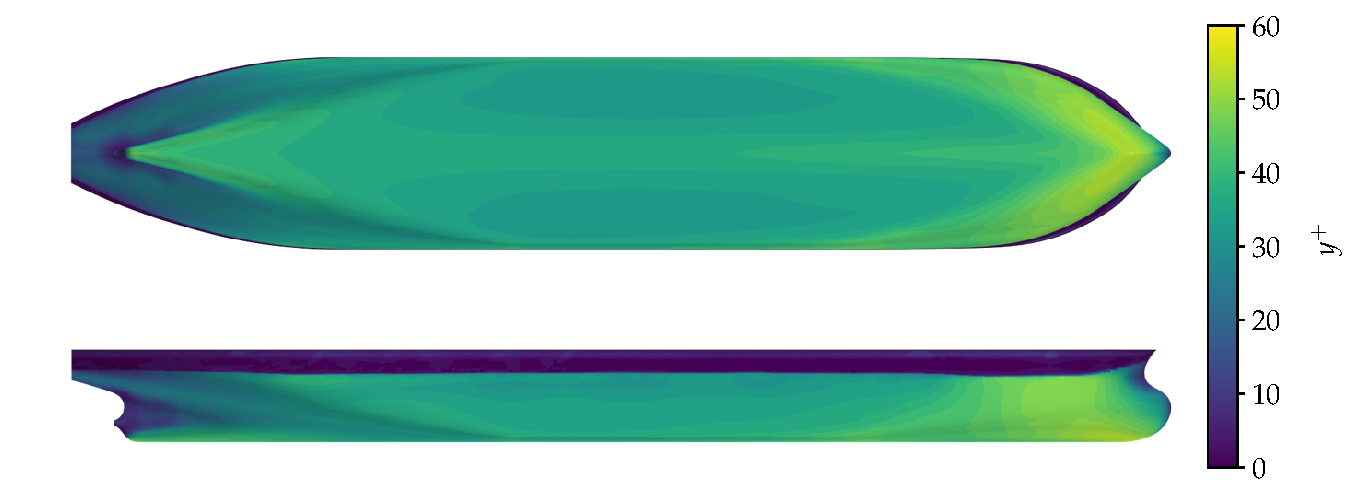
\includegraphics[width=1.0\linewidth]{yplus_0.pdf}  
	% part in the [] goes to list of table, part in {} goes to text 
	\caption{Bottom and profile view of the non-dimensional wall distance ($y^{+}$) on the KVLCC2 for the static drift simulation ($\beta=0^{\circ}$, $Fr=0.142$).}
	\label{fig:yplus}
\end{figure}
At quis risus sed vulputate. Amet risus nullam eget felis eget nunc. Ac felis donec et odio pellentesque. A iaculis at erat pellentesque adipiscing. A pellentesque sit amet porttitor. Ridiculus mus mauris vitae ultricies leo integer malesuada nunc vel. Cras semper auctor neque vitae tempus quam pellentesque. Aliquam sem fringilla ut morbi tincidunt augue interdum. Nam aliquam sem et tortor consequat id porta nibh venenatis. Nullam vehicula ipsum a arcu. Bibendum neque egestas congue quisque egestas. Quis enim lobortis scelerisque fermentum dui. Nibh ipsum consequat nisl vel pretium lectus quam id. Arcu dictum varius duis at consectetur lorem donec massa sapien. In est ante in nibh mauris. Placerat vestibulum lectus mauris ultrices eros. Sit amet aliquam id diam maecenas. Viverra vitae congue eu consequat ac. Consequat mauris nunc congue nisi vitae suscipit tellus mauris.


\begin{table}[h!]
\caption{Example of a threeparttable, useful for footnotes in tables.}
\label{tab:solver}
\centering
    \begin{threeparttable}
    	\begin{tabular}{llc}
			\toprule
			Boundary & Quantity & Value \\
			\midrule
			Inlet  & -Turbulence Intensity & 0.01 \\
				   & -Turbulent Viscosity Ratio & 10.0 \\
				   & -Velocity & Wave\tnote{1} \\
				   & -Volume Fraction & Wave\tnote{1}\\
			Outlet & -Turbulence Intensity & 0.01 \\
				   & -Turbulent Viscosity Ratio & 10.0 \\
				   & -Pressure & Wave\tnote{1} \\
				   & -Volume Fraction & Wave\tnote{1}\\
			Hull   & -Shear Stress & No-Slip\\
			Deck   & -Shear Stress & Slip\\
			Tank Walls  & -Shear Stress & Slip\\
			\bottomrule
		\end{tabular} 
    	\begin{tablenotes}
			\footnotesize
    		\item[1] Star-CCM$^{+}$ uses flat-water waves when using the VOF model to specify the velocity, hydrostatic pressure and volume fraction at the boundaries.
    	\end{tablenotes}
    \end{threeparttable}
\end{table}